% background chapter continued
\section{Software Design Principles}
This section mentions few core design principles necessary to maintain healthy codebase and knowledge to
build scalable software. The design patterns are abstract and universally applied in different programming paradigms.
\\
\\
\subsection{Open-Close Principle}
When a certain code is designed with an intent to extend it but does not need any modification
whenever requirements change or when new use-case is requested, such code is said obeying open-close
principle. In other words, it is open for extension and closed modificaiton. This design process gives
more flexibility to the program and make future changes cheaper.

\begin{figure}[h!]
  \centering
  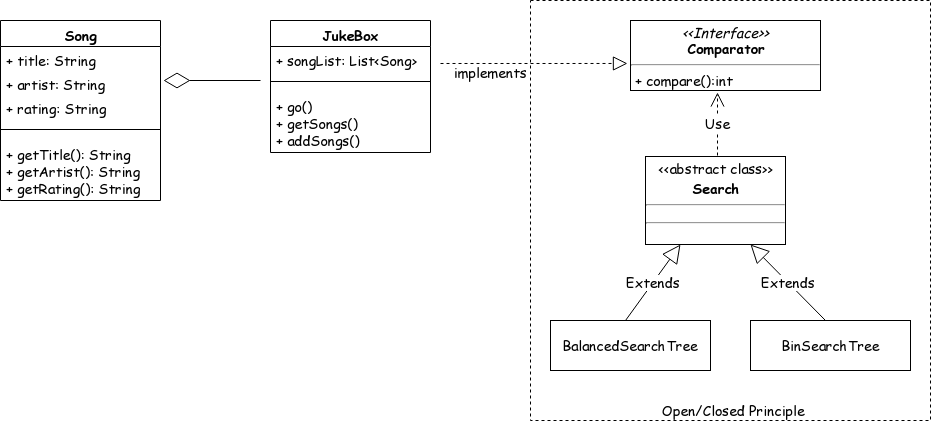
\includegraphics[width=15cm,height=12cm,keepaspectratio]{../media/crawler/opencloseprinciple.png}
  \caption{A example JukeBox program using Open/Close Principle}
  \label{fig:jukebox}
\end{figure}

\noindent
Consider an example of this principle in image \ref{fig:jukebox}, the Jukebox inner class implements Comparator interface, overriding compare method to search on different attributes of the class (eg. search on title, artist, etc). That method is invoked from concrete implementation of abstract Search class.
algorithm upon calling Collections.search(). The search functionality offered by two concrete class vary
independently and their runtime doesn't affect each other. Even more search algorithms can added without
affecting existing search. The same comparators in JukeBox can also be used to perform sorting on songs
called by respective sorting algorithm overriding sort method from sort interface.

\pagebreak

\subsection{Dependency Injection}
Dependency Injection(DI) promotes open-closed principle and reduces loose coupling. It is one of the most
important topics applicable to almost all software produced. DI provides references to objects the class
depends on instead of allowing class to gather dependencies by itself. The dependent class doesn't
take into account the how, where and what of implementation. This makes great impact on the flexibility of
software design.
\begin{figure}[h!]
  \centering
  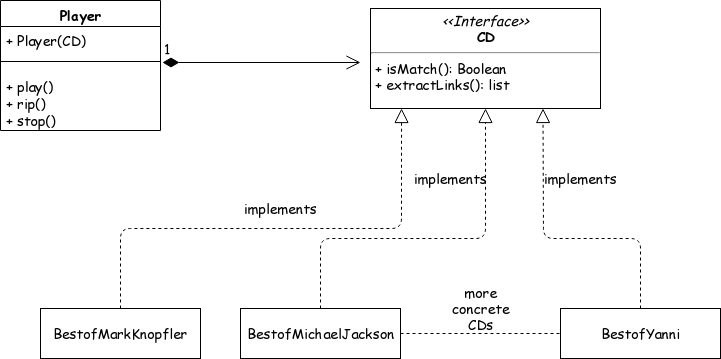
\includegraphics[width=15cm,height=12cm,keepaspectratio]{../media/crawler/dinjection.png}
  \caption{CD Player using Dependency Injection}
  \label{fig:dinjection}
\end{figure}

\noindent
Figure \ref{fig:dinjection} shows an implementation using Dependency Injection. The Player class is a dumb box; it does not know anything about Compact Disc(CDs) shown above i.e BestofMarkKnopfler, BestofMichaelJackson; it is dependent on its client to provide with working instance of CD. Without DI, the Player can
create and play only records that were harcoded in its implementation. Anytime, a new records need to be
played, Player class needs changes to its code. This violates Open-Close principle. DI makes the code
reusable and increases unit tests.

\noindent
DI can be achieved in multiple ways depending on the programming language in use. For dynamic languages
like javascript and python, the support for higher order functions can perform dependency injection
whereas static, class based language such as java, DI is achieved using DI frameworks.

\pagebreak

\subsection{Dependency Inversion}
Dependency Injection is subclass of broader principle called Dependency Inversion. Its aim is same as
DI - to make the class as simple and less coupled to the rest of the system. Inversion concept is observed
in MVC frameworks. Its promotes the philosophy of coding to contract. Contract being the creator of plugins
and not worrying who will use them; the inversion figures out which class to instantiate. It can load
dependencies on a scale of 100.
\\
\\
\noindent
Inversion is identified as `Hollywood Principle` - Don't call us, we will call you. Features found in a
piece of software supporting DI framework include:
\begin{itemize}
  \item expands code only through plugin/extensions
  \item plugins are independent and can be added or removed any point of time.
  \item system auto-detects plugins, configures which plugins should be used and how
  \item defines interface for each plugin type
\end{itemize}


\pagebreak

\subsection{Principles for designing scalable systems}
When a piece of software needs to grow to a size requiring horizontal scalability, careful thought must
be given to tradeoffs between endless scalability and practicality of each solution. Also assessment of not
overengineering the solution needs to taken into account. Here are basic design techniques that help design
scalable systems.
\\
\\
\begin{itemize}
  \item \textbf{Adding identical copies of components}
  \item \textbf{Functional partitioning}
  \item \textbf{Data partitioning}
\end{itemize}

\pagebreak

\subsection{Managing State}\label{managestate}
Managing state is often overlooked aspect when addressing the scaling problem of the application.